\chapter{Chapter 3}
\section{Introduction}
In this Chapter, we aim to  investigate   the DCA data pre-processing phase including the step of feature selection/reduction   and the step of signal categorization. We aim to detect and to handle  the shortcomings of these two steps. To do so,  we suggest to apply Rough Set Theory (RST) as a feature selection and signal categorization technique in the DCA data pre-processing phase. This will result on different DCA new automated approaches that will be compared to each other while pointing out their characteristics. 

This Chapter is organized as follows: Firstly,  criticisms of the standard DCA  data pre-processing  module are given in Section 3.2. Secondly,  the development  of the proposed  rough   pre-processing modules is based on a set of hypotheses. These hypotheses are  presented in Section   3.3. Then, the proposed rough DCA hybrid approaches are explained in details in Sections 3.4, 3.5 and 3.6.

\section{Rough DCA Based Methods}
To handle the mentioned  drawbacks of the standard DCA data pre-processing module, we propose three automated  DCAs based on the theory of rough sets (RST). The difference between the three proposed rough DCAs is based on a set of hypotheses that will be tested later in the experimental part of this Chapter. The drawn hypotheses are constructed as follows:
\begin{itemize}
\item  \textbf{H1:} The categorization of different features to different signals leads to improve the performance of the dendritic cell algorithm. We will show that assigning for each selected feature a specific signal category  leads to a better performance than assigning the same attribute to both SSs and PAMPs.
\item  \textbf{H2:} The use of a rough set heuristic  can keep the DCA main characteristic which is its lightweight in terms of processing time. This will be achieved by finding a trade-off between generating satisfactory classification results and preserving the lightweight of the algorithm.
\end{itemize}

H1 focuses on checking whether designating the same attribute to both SSs and PAMPs is more convenient for the DCA signal categorization substep than assigning different features for each signal category. By designating the same attribute to both SSs and PAMPs, we develop our first  DCA model based on Rough Set Theory (RST) named RST-DCA. By attaching different attributes to different signals, we develop our second rough DCA model   based on the  ``Reduct" and the ``Core" RST concepts. The proposed algorithm is  named RC-DCA. Conversely, H2 deals with the development of our third rough DCA    based on the use of a rough heuristic; i.e.,  the QuickReduct algorithm. The proposed rough DCA   is named QR-DCA. By developing the latter algorithm, we try to find a trade-off between generating satisfactory classification results and preserving the lightweight of the standard DCA.
\begin{figure}[!h]
\begin{center}
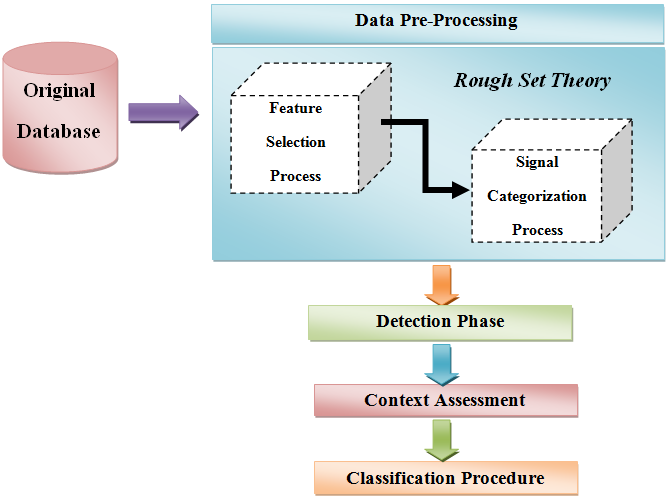
\includegraphics[width=8cm,height=7cm]{RSTModel}
\caption{The Rough DCA Proposed Model}\label{steps}
\end{center}
\end{figure}

The three developed rough DCAs, including  RST-DCA, RC-DCA and QR-DCA,  function under four levels of abstraction as shown in Figure \ref{steps}. We will mainly discuss the algorithms data pre-processing phase  as the rest of the algorithms steps are performed the same as the standard DCA and as explained, previously, in Chapter 1.

\section{Conclusion}
In this Chapter, we have elucidated  how rough set theory could be used to select the right features  and to categorize each selected attribute to its signal category. We have developed three rough dendritic cell algorithms, compared them and noted the appropriate observations while testing two crucial hypotheses. 

Despite of the noticed advantages of our proposed rough set methods, they have some limitations when dealing with real-valued attributes. This prompted our research into the use of fuzzy-rough sets for feature selection and signal categorization. This will be dealt with in the next Chapter.
